\documentclass[fleqn]{article}
\usepackage[nodisplayskipstretch]{setspace}
\usepackage{amsmath, nccmath}
\usepackage{amssymb}
\usepackage{enumitem}
\usepackage{matlab-prettifier}
\usepackage{scalerel}
\usepackage{graphicx}
\usepackage{float}
\usepackage{changepage}
\usepackage{environ,capt-of}

\newcommand{\zerodisplayskip}{
	\setlength{\abovedisplayskip}{0pt}%
	\setlength{\belowdisplayskip}{0pt}%
	\setlength{\abovedisplayshortskip}{0pt}%
	\setlength{\belowdisplayshortskip}{0pt}%
	\setlength{\mathindent}{0pt}}
	
\let\oldfigure\figure% Store original figure float environment
\let\endoldfigure\endfigure
\RenewEnviron{figure}[1][H]{% Update figure environment
  %\par\vspace{\intextsep}% Assume in-text placement, so insert appropriate vertical spacing
  \noindent
  % \patchcmd{<cmd>}{<search>}{<replace>}{<success>}{<failure>}
  \patchcmd{\BODY}{\caption}{\captionof{figure}}{}{}% Replace \caption with \captionof{figure} inside \BODY
  % Set "figure"
  \begin{minipage}{\linewidth}
    \BODY
  \end{minipage}
  %\par\vspace{\intextsep}% Assume in-text placement, so insert appropriate vertical spacing
}

\title{Homework 5}
\author{Owen Sowatzke}
\date{November 16, 2023}

\begin{document}
	\offinterlineskip
	\setlength{\lineskip}{12pt}
	\zerodisplayskip
	\maketitle
	
	\begin{enumerate}[nolistsep]
		\item Design a discrete-time second-order Butterworth lowpass filter with cutoff frequency equivalent to $f_c = 1.6 \text{kHz}$. Assume the ADC sampling frequency is $f_s = 8 \text{kHz}$. Use the impulse invariance method with $T_d = 1$.
		
			\begin{enumerate}[nolistsep]
				\item Calculate the cutoff frequency for the desired digital filter (i.e., convert the analog specs to digital specs.)
				
					\begin{equation*}
						\omega_c = \frac{2{\pi}f_c}{f_s} = \frac{2{\pi}(1.6\ \text{kHz})}{8\ \text{kHz}} = \mathbf{0.4\pi}
					\end{equation*}
					
				\item Calculate the cutoff frequency for the prototype analog filter.
				
					\begin{equation*}
						\Omega_c = \frac{\omega_c}{T_d} = \mathbf{0.4\pi\ \text{\textbf{rad/s}}} 
					\end{equation*}
					
				\item Derive the transfer function $H_a(s)$ for the prototype analog filter by selecting the left-half-plane poles of $H_a(s)H_a(-s)$. Show your work. Show that this matched the result of the following MATLAB command:
				
				\texttt{[bs, as] = butter(N,$\Omega_c$,'low','s')}
				
				\begin{equation*}
					H_a(s)H_a(-s) = \frac{(-1)^N{\Omega_c}^{2N}}{s^{2N} + (-1)^N{\Omega_c}^{2N}}
				\end{equation*}
				
				\begin{equation*}
					= \frac{(-1)^2(0.4\pi)^4}{s^4 + (-1)^4(0.4\pi)^4} = \frac{(0.4\pi)^4}{s^4 + (0.4\pi)^4}
				\end{equation*}
				
				Solve for the poles of the above expression:
				
				$s^4 + (0.4\pi)^4 = 0$
				
				$\Rightarrow s^4 = -(0.4\pi)^4$
				
				$\Rightarrow s^4 = (0.4\pi)^4e^{j\pi}$
				
				$\Rightarrow s^4 = (0.4\pi)^4e^{j(\pi + 2{\pi}k)}\ \forall\ k \in \mathbb{Z}$
				
				$\Rightarrow s = 0.4{\pi}e^{j({\pi/4} + {\pi}k/2)}\ \forall\ k \in \mathbb{Z}$
				
				$\therefore$ $H_a(s)H_a(-s)$ has 4 unique poles:
				
				$s_1 = 0.4{\pi}e^{j{\pi}/4}$
				
				$s_2 = 0.4{\pi}e^{j3{\pi}/4}$
				
				$s_3 = 0.4{\pi}e^{-j3{\pi}/4}$
				
				$s_4 = 0.4{\pi}e^{-j{\pi}/4}$
				
				Because the filter is stable, the poles of $H_a(s)$ must be in the LHP.
				
				$\therefore$ $H_a(s)$ has two poles:
				
				$s_1 = 0.4{\pi}e^{j3{\pi}/4}$
				
				$s_2 = 0.4{\pi}e^{-j3{\pi}/4}$
				
				Now, we can rewrite $H_a(s)$ in the following form:
				
				\begin{equation*}
					H_a(s) = \frac{(0.4\pi)^2}{(s - 0.4{\pi}e^{j3{\pi}/4})(s - 0.4{\pi}e^{-j3{\pi}/4})}
				\end{equation*}
				
				\begin{equation*}
					= \frac{(0.4\pi)^2}{s^2 - (0.4{\pi}e^{j3{\pi}/4} + 0.4{\pi}e^{-j3{\pi}/4})s + (0.4\pi)^2}
				\end{equation*}
				
				\begin{equation*}
					= \frac{(0.4\pi)^2}{s^2 - 0.8\pi\cos(3\pi/4)s + (0.4\pi)^2}
				\end{equation*}
				
				\begin{equation*}
					\mathbf{= \frac{1.5791}{s^2 + 1.7772s + 1.5791}}
				\end{equation*}
				
				\pagebreak
				We can compare this transfer function to the output of the following MATLAB command:
				
				\begin{figure}[H]
					\centerline{\fbox{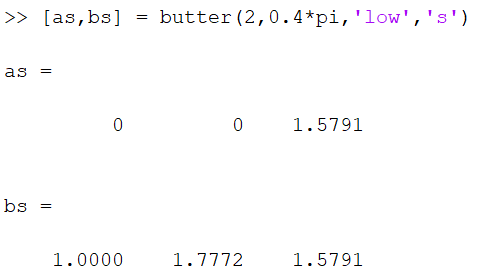
\includegraphics[width=0.5\textwidth]{prob_1c.png}}}
					\caption{Using MATLAB to Solve for $H_a(s)$}
				\end{figure}
				
				The transfer function $H_a(s)$ derived using MATLAB has numerator polynomial of $0s^2 + 0s + 1.5791 = 1.5971$ and a denominator polynomial of $s^2 + 1.7772s + 1.5791$. Note that this is equivalent to the transfer function that was analytically derived.
				
				\item Derive the transfer function $H(z)$ for the desired digital filter. Also show the result of the following MATLAB command, which gives the coefficients for the final, simplified $H(z)$:
				
				\texttt{[bz, az] = impinvar(bs,as,$1/T_d$)}
				
				We first need to find $h_a(t)$ by taking an inverse Laplace transform of $H_a(s)$. Start by using partial fraction expansion to write $H_a(s)$ in the following form:
				
				\begin{equation*}
					H_a(s) = \frac{A_1}{s - 0.4{\pi}e^{j3{\pi}/4}} +  \frac{A_2}{s - 0.4{\pi}e^{-j3{\pi}/4}}
				\end{equation*}
				
				\begin{equation*}
					A_1 = H_a(s)(s - 0.4{\pi}e^{j3{\pi}/4}) = \left.\frac{(0.4\pi)^2}{s - 0.4{\pi}e^{-j3{\pi}/4}}\right\vert_{s = 0.4{\pi}e^{j3{\pi}/4}}
				\end{equation*}
				
				\begin{equation*}
					= \frac{(0.4\pi)^2}{0.4{\pi}e^{j3{\pi}/4} - 0.4{\pi}e^{-j3{\pi}/4}} = \frac{(0.4\pi)^2}{j0.8{\pi}\sin(3\pi/4)}
				\end{equation*}
				
				\begin{equation*}
					 = \frac{(0.4\pi)}{j2(1/\sqrt{2})} = -\frac{j\pi\sqrt{2}}{5}
				\end{equation*}
				
				\begin{equation*}
					A_2 = H_a(s)(s - 0.4{\pi}e^{-j3{\pi}/4}) = \left.\frac{(0.4\pi)^2}{s - 0.4{\pi}e^{j3{\pi}/4}}\right\vert_{s = 0.4{\pi}e^{-j3{\pi}/4}}
				\end{equation*}
				
				\begin{equation*}
					= \frac{(0.4\pi)^2}{0.4{\pi}e^{-j3{\pi}/4} - 0.4{\pi}e^{j3{\pi}/4}} = \frac{(0.4\pi)^2}{-j0.8{\pi}\sin(3\pi/4)}
				\end{equation*}
				
				\begin{equation*}
					 = \frac{(0.4\pi)}{-j2(1/\sqrt{2})} = \frac{j\pi\sqrt{2}}{5}
				\end{equation*}
				
				\begin{equation*}
					H_a(s) = \frac{-j\pi\sqrt{2}}{5}\left(\frac{1}{s - 0.4{\pi}e^{j3\pi/4}}\right) + \frac{j\pi\sqrt{2}}{5}\left(\frac{1}{s - 0.4{\pi}e^{-j3\pi/4}}\right)
				\end{equation*}
				
				\begin{equation*}
					= \frac{-j\pi\sqrt{2}}{5}\left(\frac{1}{s - 0.4{\pi}\left(-\frac{1}{\sqrt{2}} + \frac{j}{\sqrt{2}}\right)}\right)
				\end{equation*}
				
				\begin{equation*}
					 + \frac{j\pi\sqrt{2}}{5}\left(\frac{1}{s - 0.4{\pi}\left(-\frac{1}{\sqrt{2}} - \frac{j}{\sqrt{2}}\right)}\right)
				\end{equation*}
				
				Now take the inverse Laplace transform to get $h_a(t)$.
				
				\begin{equation*}
					h_a(t) = \frac{-j\pi\sqrt{2}}{5}e^{0.4\pi\left(-\frac{1}{\sqrt{2}} + \frac{j}{\sqrt{2}}\right)t}u(t) + \frac{j\pi\sqrt{2}}{5}e^{0.4\pi\left(-\frac{1}{\sqrt{2}} - \frac{j}{\sqrt{2}}\right)t}u(t)
				\end{equation*}
				
				\begin{equation*}
					= \frac{\pi\sqrt{2}}{5}e^{-\frac{0.4{\pi}t}{\sqrt{2}}}\left(-je^{\frac{j0.4{\pi}t}{\sqrt{2}}} + je^{-j\frac{0.4{\pi}t}{\sqrt{2}}}\right)u(t)
				\end{equation*}
				
				\begin{equation*}
					= \frac{2\pi\sqrt{2}}{5}e^{-\frac{0.4{\pi}t}{\sqrt{2}}}\left(\frac{e^{\frac{j0.4{\pi}t}{\sqrt{2}}} - e^{-\frac{j0.4{\pi}t}{\sqrt{2}}}}{j2}\right)u(t)
				\end{equation*}
				
				\begin{equation*}
					 = \frac{2\pi\sqrt{2}}{5}e^{-\frac{0.4{\pi}t}{\sqrt{2}}}\sin{\left(\frac{0.4{\pi}t}{\sqrt{2}}\right)}u(t)
				\end{equation*}
				
				Now sample $h_a(t)$ to obtain $h[n]$:
				
				\begin{equation*}
					h[n] = \frac{2\pi\sqrt{2}}{5}e^{-\frac{0.4{\pi}n}{\sqrt{2}}}\sin{\left(\frac{0.4{\pi}n}{\sqrt{2}}\right)}u[n]
				\end{equation*}
				
				Use the following z-transform pair to obtain $H(z)$
				
				\begin{equation*}
					r^{n}sin({\omega_0}n)u[n] \leftrightarrow \frac{rsin(\omega_0)z^{-1}}{1 - 2rcos(\omega_0)z^{-1} + r^{2}z^{-2}}\quad |z| > r
				\end{equation*}
				
				\begin{equation*}
					H(z) = \frac{2\pi\sqrt{2}}{5}\left(\frac{e^{-\frac{0.4\pi}{\sqrt{2}}}\sin{\left(\frac{0.4\pi}{\sqrt{2}}\right)z^{-1}}}{1 - 2e^{-\frac{0.4\pi}{\sqrt{2}}}\cos{\left(\frac{0.4\pi}{\sqrt{2}}\right)}z^{-1} + e^{-\frac{0.8\pi}{\sqrt{2}}}z^{-2}}\right)
				\end{equation*}
				
				\begin{equation*}
					\mathbf{= \frac{0.5673z^{-1}}{1 - 0.5186z^{-1} + 0.1691z^{-2}}}
				\end{equation*}
				
				We can compare this transfer function to the output of the following MATLAB command, where \texttt{bs} and \texttt{as} are derived are derived using the MATLAB code given in part (c):
				
				\begin{figure}[H]
					\centerline{\fbox{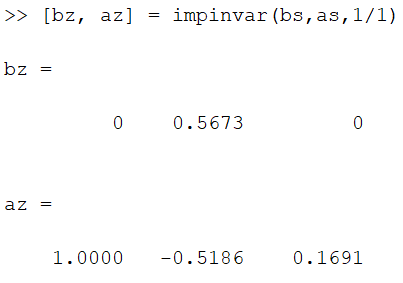
\includegraphics[width=0.5\textwidth]{prob_1d.png}}}
					\caption{Using MATLAB to Solve for $H(z)$}
				\end{figure}
				
				The transfer function $H(z)$ derived using MATLAB has numerator polynomial of $0z^{-2} + 0.5673z^{-1} + 0z^{-2} = 0.5673z^{-1}$ and a denominator polynomial of $1 - 0.5186z^{-1} + 0.1691z^{-2}$. Note that this is equivalent to the analytically-derived transfer function.
				
			\item Derive the difference equation (LCCDE) that we would use to implement the filter.
			
				$Y(z)(1 - 0.5186z^{-1} + 0.1691z^{-2}) = X(z)(0.5673z^{-1})$
				
				$y[n] - 0.5186y[n-1] + 0.1691y[n-2] = 0.5673x[n-1]$
				
				$\mathbf{y[n] = 0.5186y[n-1] - 0.1691y[n-2] + 0.5673x[n-1]}$
				
			\item Plot the frequency response as follows:
			
				\texttt{[H,w] = freqz(bz,az)}
				
				\texttt{semilogy(w/pi,abs(H))}
				
				\begin{figure}[H]
					\centerline{\fbox{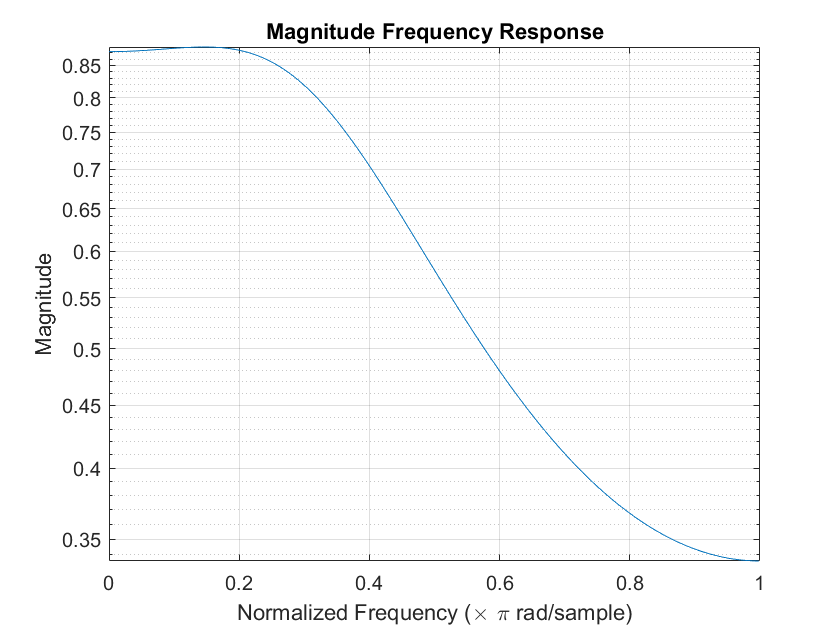
\includegraphics[width=0.5\textwidth]{prob_1f.png}}}
					\caption{Magnitude Frequency Response}
				\end{figure}
				
			\item What is the approximate magnitude frequency response at zero frequency? How can we modify the filter to achieve unit magnitude frequency response at zero frequency? Optional can you determine a way to modify the filter that will achieve unit magnitude frequency response at zero frequency without affecting the frequency response at other frequencies?
			
				The magnitude frequency response at zero frequency is approximately $0.871994$. To achieve a unit magnitude frequency response at zero frequency we want to scale the transfer function by $1/0.871994 = 1.1468$. This is equivalent to scaling the numerator of the transfer function, \texttt{bz}, by $1.1468$. This modified filter can be implemented with the following LCCDE:
				
				$y[n] = 0.5186y[n-1] - 0.1691y[n-2] + 0.6506x[n-1]$
		\end{enumerate}
		
		\item Design a discrete-time second-order Butterworth lowpass filter with cutoff frequency $\omega_c = 0.4\pi\ \text{rad}$. Use the impulse invariance method.
			Hint: This problem is trivial after you've completed the previous problem.
			
		\pagebreak
		We designed a digital filter with a cutoff frequency of $\omega_c = 0.4\pi$ in problem 1. The value chosen for $T_d$ does not influence the results. $\therefore$ regardless of which value of $T_d$ is chosen, we will end up with the same digital filter designed in problem 1. Assuming the filter is scaled to produce \newline $H(e^{j\pi}) = 1$, the transfer function of the resulting filter will be
		
		\begin{equation*}
			\mathbf{H(z) = \frac{0.6506z^{-1}}{1 - 0.51856z^{-1} + 0.1691z^{-2}}}
		\end{equation*}
		
		The resulting filter can also be implemented using the following LCCDE:
		
		$\mathbf{y[n] = 0.5186y[n-1] - 0.1691y[n-2] + 0.6506x[n-1]}$
		
		\item Design a discrete-time second-order Butterworth lowpass filter with cutoff frequency equivalent to $f_c = 1.6\ \text{kHz}$. Assume the ADC sampling frequency is $f_s = 8 \text{kHz}$. Use the bilinear transformation methods with $T_d = 2$.
		
		\begin{enumerate}
		
			\item Calculate the cutoff frequency for the desired digital filter (i.e., convert the analog specs to digital specs.)
			
			\begin{equation*}
				\omega_c = \frac{2{\pi}f_c}{f_s} = \frac{2{\pi}(1.6\ \text{kHz})}{8\ \text{kHz}} = \mathbf{0.4\pi}
			\end{equation*}
			
			\item Calculate the cutoff frequency for the prototype analog filter.
			
			\begin{equation*}
				\Omega_c = \frac{2}{T_d}\tan{\left(\frac{\omega_c}{2}\right)} = \tan{\left(\frac{0.4\pi}{2}\right)} = \tan{(0.2\pi)} = \mathbf{0.7265\ \text{\textbf{rad/s}}}
			\end{equation*}
			
			\item Show the transfer function $H_a(s)$ for the prototype analog filter.
			
			A second order butterworth filter with cutoff frequency $\Omega_c = 1\ \text{rad/s}$ has the following transfer function:
			
			\begin{equation*}
				H(s) = \frac{1}{s^2 + \sqrt{2}s + 1}
			\end{equation*}
			
			\pagebreak
			If we replace all instances of $s$ with $\frac{s}{\Omega_c}$, we can compute the transfer function $H_a(s)$
			
			\begin{equation*}
				H_a(s) = \frac{1}{\left(\frac{s}{\Omega_c}\right)^2 + \sqrt{2}\left(\frac{s}{\Omega_c}\right) + 1} = \frac{\Omega_c^2}{s^2 + \Omega_c\sqrt{2}s + \Omega_c^2}
			\end{equation*}
			
			\begin{equation*}
				= \frac{0.7265^2}{s^2 + 0.7265\sqrt{2}s + 0.7265^2} = \mathbf{\frac{0.5278}{s^2 + 1.0274s + 0.5278}}
			\end{equation*}
			
			\item Derive the transfer function $H(z)$ for the desired digital filter. Also show the result of the following MATLAB command, which gives the coefficients for the final $H(z)$:
			
			\texttt{[bz,az] = bilinear(bs,as,$1/T_d$)}
			
			$H_a(s)$ is mapped to $H(z)$ by the following substitution:
			
			\begin{equation*}
				s = \frac{2}{T_d}\left(\frac{1 - z^{-1}}{1 + z^{-1}}\right) = \frac{1 - z^{-1}}{1 + z^{-1}}
			\end{equation*}
			
			\begin{equation*}
				H(z) = \frac{0.5278}{\left(\frac{1 - z^{-1}}{1 + z^{-1}}\right)^2 + 1.0274\left(\frac{1 - z^{-1}}{1 + z^{-1}}\right) + 0.5278}
			\end{equation*}
			
			\begin{equation*}
				= \frac{0.5278(1 + z^{-1})^2}{(1 - z^{-1})^2 + 1.0274(1 - z^{-1})(1 + z^{-1}) + 0.5278(1 + z^{-1})^2}
			\end{equation*}
			
			\begin{equation*}
				= \frac{0.5278(1 + 2z^{-1} + z^{-2})}{1 - 2z^{-1} + z^{-2} + 1.0274(1 - z^{-2}) + 0.5278(1 + 2z^{-1} + z^{-2})}
			\end{equation*}
			
			\begin{equation*}
				= \frac{0.5278 + 1.0556z^{-1} + 0.5278z^{-2}}{2.5552 - 0.9444z^{-1} + 0.5004z^{-2}}
			\end{equation*}
			
			\begin{equation*}
				\mathbf{= \frac{0.2066 + 0.4131^{-1} + 0.2066z^{-2}}{1 - 0.3696z^{-1} + 0.1958z^{-2}}}
			\end{equation*}
			
			\pagebreak
			We can validate the transfer function using the following MATLAB code:
			
			\begin{figure}[H]
					\centerline{\fbox{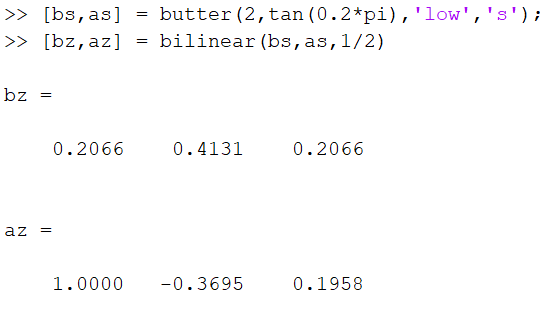
\includegraphics[width=0.5\textwidth]{prob_3d.png}}}
					\caption{Using MATLAB to Solve for $H(z)$}
			\end{figure}
			
			The transfer function $H(z)$ derived using MATLAB has numerator polynomial of $0.2066 + 0.4131z^{-1} + 0.2066z^{-2}$ and a denominator polynomial of $1 - 0.3695z^{-1} + 0.1958z^{-2}$. Note that this is approximately the same as the analytically-derived transfer function. Any differences in the transfer function are due to round-off errors in the analytic calculation.
			
			\item Derive the difference equation (LCCDE) that we would use to implement the filter.
			
			\begin{equation*}
				Y(z)(1 - 0.3696z^{-1} + 0.1958z^{-2})
			\end{equation*}
			
			\begin{equation*}			
				= X(z)(0.2066 + 0.4131z^{-1} + 0.2066z^{-2})
			\end{equation*}
			
			\begin{equation*}
				y[n] - 0.3696y[n-1] + 0.1958y[n-2]
			\end{equation*}
			
			\begin{equation*}
				 = 0.2066x[n] + 0.4131x[n-1] + 0.2066x[n-2]
			\end{equation*}
			
			\begin{equation*}
				\mathbf{y[n] = 0.3696y[n-1] - 0.1958y[n-2]}
			\end{equation*}
			
			\begin{equation*}
				\mathbf{+ 0.2066x[n] + 0.4131x[n-1] + 0.2066x[n-2]}
			\end{equation*}
			
			\pagebreak
			\item Plot the frequency response as follows:
			
			\texttt{[H,w] = freqz(bz,az)}
			
			\texttt{semilogy(w/pi,abs(H))}
			
			What is the approximate magnitude frequency response at zero frequency? How does the frequency response at $\omega = \pi$ compare with the corresponding frequency response observed in Problem 1?
			
			\begin{figure}[H]
					\centerline{\fbox{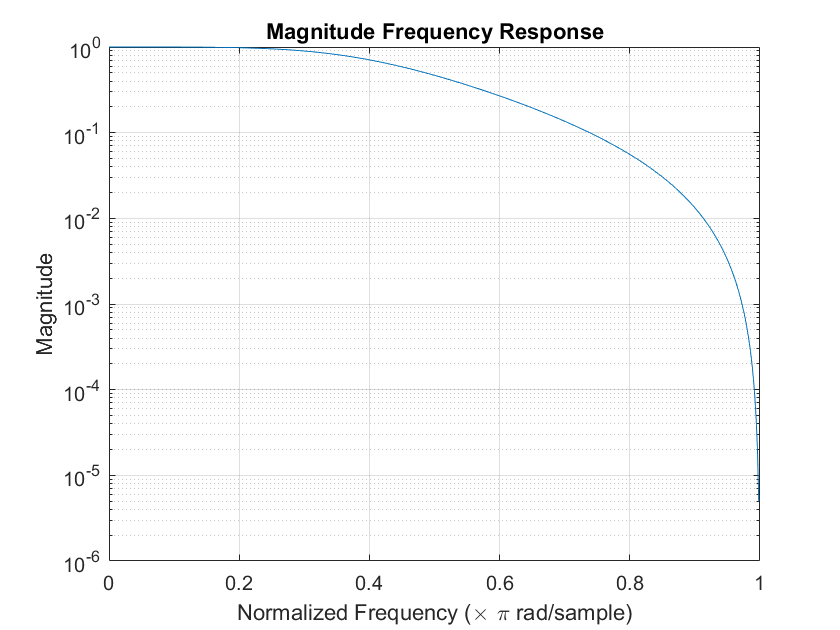
\includegraphics[width=0.5\textwidth]{prob_3f.png}}}
					\caption{Magnitude Frequency Response}
			\end{figure}
			
			The magnitude frequency response at zero frequency is $1$. The magnitude frequency response at $\omega = \pi$ is $-\infty$. The magnitude frequency response is $-\infty$ at $\omega=\pi$ because the bilinear transform maps the entire $j\Omega$-axis in the s-plane to one revolution of the unit circle in the z-plane. Compare this to the magnitude frequency response of the filter in Problem 1 which is approximately $0.3361$ at $\omega = \pi$. Compared to the bilinear transform, the impulse invariance method only maps a portion of the analog frequency response [-$\pi/T_d$, $\pi/T_d$) to a revolution of the unit circle in the z-plane. The rest of frequency response aliases.
			
			\item The \texttt{butter()} function can also be used to directly design a discrete-time filter using the bilinear transformation by omitting the final \texttt{'s'} parameter and specifying the cutoff frequency as a normalized digital frequency between 0 and 1:
			
			\texttt{[bz,az] = butter(N,$\omega_c$(normalized),'low')}
			
			Show that this produces the same result as in part (d).
			
			\begin{figure}[H]
					\centerline{\fbox{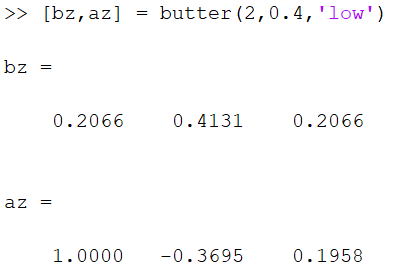
\includegraphics[width=0.5\textwidth]{prob_3g.png}}}
					\caption{Using MATLAB to Solve for $H(z)$}
			\end{figure}
				
			The arrays \texttt{az} and \texttt{bz} computed using the above command match the values computed in part (d).
		\end{enumerate}
		
		\item Design a discrete-time second-order Butterworth lowpass filter with cutoff frequency $\omega_c = 0.4\pi\ \text{rad}$. Use the bilinear transform method.
		
		Hint: This problem is trivial after you've completed the previous problem.
		
		\item An ideal discrete-time highpass filter with $\omega_c = 3\pi/4$ is given by
		
		\begin{equation*}
			H_d(e^{j\omega}) = 
			\begin{cases}
				0, & |\omega| < 3\pi/4 \\
				1, & 3\pi/4 < |\omega| \leq \pi
			\end{cases}
		\end{equation*}
		
		Use the window method to design a zero-phase FIR filter that approximates $H_d(e^{j\omega})$. Use a rectangular window of length 5. Show the transfer function $H(z)$ of the resulting filter. Evaluate the expressions to obtain the numerical values. Scale the filter so that the frequency response is one at $\omega = \pi$. Note that $H(e^{j\pi}) = \sum_{n}{h(n)e^{-j{\pi}n}} = \sum_{n}{h(n)(-1)^n}$.
		
		Find the impulse response of the ideal highpass filter:
		
		\begin{equation*}
			h_d[n] = \frac{1}{2\pi}\int_{-\pi}^{\pi}{H_d(e^{j\omega})e^{j{\omega}n}}d\omega
		\end{equation*}
		
		\begin{equation*}
			= \frac{1}{2\pi}\left(\int_{-\pi}^{-3\pi/4}{e^{j{\omega}n}d\omega} + \int_{3\pi/4}^{\pi}{e^{j{\omega}n}d\omega}\right)
		\end{equation*}
		
		\begin{equation*}
			= \frac{1}{2\pi}\left(\left.\frac{e^{j{\omega}n}}{jn}\right\vert_{-\pi}^{-3\pi/4} + \left.\frac{e^{j{\omega}n}}{jn}\right\vert_{3\pi/4}^{\pi}\right)
		\end{equation*}
		
		\begin{equation*}
			= \frac{1}{2\pi}\left(\frac{e^{-j3{\pi}n/4} - e^{-j{\pi}n}}{jn} + \frac{e^{j{\pi}n} - e^{j3{\pi}n/4}}{jn}\right)
		\end{equation*}
		
		\begin{equation*}
			= \frac{1}{{\pi}n}\left(\frac{e^{j{\pi}n} - e^{-j{\pi}n}}{j2} - \frac{e^{j3{\pi}n/4} - e^{-j3{\pi}n/4}}{j2}\right)
		\end{equation*}
		
		\begin{equation*}
			= \frac{\sin{({\pi}n)} - \sin{(3{\pi}n/4)}}{{\pi}n} \quad {\text{if}}\ n \neq 0
		\end{equation*}
		
		\begin{equation*}
			h_d[0] = \frac{1}{2\pi}\int_{-\pi}^{\pi}{H_d(e^{j\omega})d\omega}
		\end{equation*}
		
		\begin{equation*}
			= \frac{1}{2\pi}\left(\int_{-\pi}^{-3\pi/4}{d\omega} + \int_{3\pi/4}^{\pi}{d\omega}\right)
		\end{equation*}
		
		\begin{equation*}
			= \frac{1}{2\pi}\left(\left.\omega\right\vert_{-\pi}^{-3\pi/4} + \left.\omega\right\vert_{3\pi/4}^{\pi}\right)
		\end{equation*}
		
		\begin{equation*}
			= \frac{1}{2\pi}\left(-\frac{3\pi}{4} - (-\pi) + \pi - \frac{3\pi}{4}\right)
		\end{equation*}
		
		\begin{equation*}
			= \frac{1}{2\pi}\left(\frac{\pi}{2}\right) = \frac{1}{4}
		\end{equation*}
		
		\begin{equation*}
			h_d[n] =
			\begin{cases}
				\frac{\sin{({\pi}n)} - \sin{(3{\pi}n/4)}}{{\pi}n}, & n \neq 0 \\
				\frac{1}{4}, & n = 0
			\end{cases}
		\end{equation*}
		
		The window function is defined by the following formula:
		
		$w[n] = u[n] - u[n - 5]$
		
		If the window function is centered about $n = 0$ and multiplied with $h_d[n]$, we can obtain the impulse response, $h[n]$.
		
		$h[n] = h_d[n]w[n + 2]$
		
		\begin{equation*}
			h[n] =
			\begin{cases}
				0.25, & n = 0 \\
				-0.2251, & |n| = 1 \\
				0.1592, & |n| = 2\\
				0, & \text{otherwise}
			\end{cases}
		\end{equation*}
		
		$h[n] = 0.1592\delta[n+2] - 0.2251\delta[n+1] + 0.25\delta[n]$
		
		$ - 0.2251\delta[n-1] +  0.1592\delta[n-2]$
		
		Determine scaling required to make $H(e^{j\pi}) = 1$:
		
		\begin{equation*}
			H(e^{j\pi}) = \sum_{n=-\infty}^{\infty}{h[n]e^{-j{\pi}n}} = \sum_{n=-\infty}^{\infty}{h[n](-1)^n}
		\end{equation*}
		
		\begin{equation*}
			= 0.1592(-1)^{-2} - 0.2251(-1)^{-1} + 0.25(-1)^{0} - 0.2251(-1)^{1} +  0.1592(-1)^{2}
		\end{equation*}
		
		\begin{equation*}
			= 0.1592 + 0.2251 + 0.25 + 0.2251 + 0.1592 = 1.0186
		\end{equation*}
		
		Scale the coefficients by $1/1.0186$ to make $H(e^{j\pi}) = 1$.
		
		\begin{equation*}
			h[n] = \frac{1}{1.0186}(0.1592\delta[n+2] - 0.2251\delta[n+1] + 0.25\delta[n]
		\end{equation*}
		
		$- 0.2251\delta[n-1] +  0.1592\delta[n-2])$
		
		$\Rightarrow h[n] = 0.1562\delta[n+2] - 0.2210\delta[n+1] + 0.2454\delta[n]$
		
		$- 0.2210\delta[n-1] +  0.1562\delta[n-2])$
		
		Take the z-transform to obtain $H(z)$:
		
		$\mathbf{H(z) = 0.1562z^2 - 0.2210z + 0.2454 - 0.2210z^{-1} +  0.1562z^{-2}}$
		
		\pagebreak
		\item Design an anti-symmetric FIR highpass filter with length $4$ and digital cutoff frequency $\omega_c = 0.4\pi$. Use a Hamming window. Show the transfer function $H(z)$ of the resulting filter. Evaluate the expressions to obtain the numerical values. Scale the filter so that the frequency response is one at $\omega = \pi$. Note that $H(e^{j\pi}) = \sum_{n}{h(n)e^{-j{\pi}n}} = \sum_{n}{h(n)(-1)^n}$.
		
		Ideal frequency response:
		
		\begin{equation*}
			H_d(e^{j\omega}) =
			\begin{cases}
				j, & 0.4\pi < \omega \leq \pi \\
				0, & -0.4\pi \leq \omega \leq 0.4\pi \\
				-j, & -\pi \leq \omega < -0.4\pi
			\end{cases}
		\end{equation*}
		
		Compute the ideal impulse response:
		
		\begin{equation*}
			h_d[n] = \frac{1}{2\pi}\int_{-\pi}^{\pi}{H_d(e^{j\omega})e^{j{\omega}n}d\omega}			
		\end{equation*}
		
		\begin{equation*}
			= \frac{1}{2\pi}\left(\int_{-\pi}^{-0.4\pi}{-je^{j{\omega}n}d\omega} + \int_{0.4\pi}^{\pi}{je^{j{\omega}n}d\omega}\right)		
		\end{equation*}
		
		\begin{equation*}
			= \frac{1}{2\pi}\left(-\left.\frac{e^{j{\omega}n}}{n}\right\vert_{-\pi}^{-0.4\pi} + \left.\frac{e^{j{\omega}n}}{n}\right\vert_{0.4\pi}^{\pi}\right)		
		\end{equation*}
		
		\begin{equation*}
			= \frac{1}{2\pi}\left(-\frac{e^{-j0.4{\pi}n}}{n} + \frac{e^{-j{\pi}n}}{n} + \frac{e^{j{\pi}n}}{n} - \frac{e^{j0.4{\pi}n}}{n}\right)		
		\end{equation*}
		
		\begin{equation*}
			= \frac{1}{{\pi}n}\left(\frac{e^{j{\pi}n} + e^{-j{\pi}n}}{2} - \frac{e^{j0.4{\pi}n} + e^{-j0.4{\pi}n}}{2}\right)		
		\end{equation*}
		
		\begin{equation*}
			= \frac{\cos{({\pi}n)} - cos{(0.4{\pi}n)}}{{\pi}n}\quad \text{if}\ n \neq 0
		\end{equation*}
		
		\begin{equation*}
			h_d[0] = \frac{1}{2\pi}\int_{-\pi}^{\pi}{H_d(e^{j\omega})d\omega}			
		\end{equation*}
		
		\begin{equation*}
			= \frac{1}{2\pi}\left(\int_{-\pi}^{-0.4\pi}{-jd\omega} + \int_{0.4\pi}^{\pi}{jd\omega}\right)
		\end{equation*}
				
		\begin{equation*}
			= \frac{1}{2\pi}\left(\left.-j\omega\right\vert_{-\pi}^{-0.4\pi} + \left.j\omega\right\vert_{0.4\pi}^{\pi}\right)
		\end{equation*}
		
		\begin{equation*}
			= \frac{1}{2\pi}\left(j0.4\pi - j\pi + j\pi - j0.4\pi\right) = 0
		\end{equation*}
		
		\begin{equation*}
			h_d[n] =
			\begin{cases}
				\frac{\cos{({\pi}n)} - cos{(0.4{\pi}n)}}{{\pi}n}, & n \neq 0 \\
				0, & n = 0
			\end{cases}
		\end{equation*}
		
		The window function is defined by the following formula:
		
		\begin{equation*}
			w[n] =
			\begin{cases}
				0.54 - 0.46\cos{\left(\frac{2{\pi}n}{N - 1}\right)}, & 0 \leq n \leq 3 \\
				0, & \text{otherwise}
			\end{cases}
		\end{equation*}
		
		Because the filter length is even, we cannot design a zero-phase FIR filter. However, we can still design a causal FIR filter, by shifting the impulse response and multiplying it by the window.
		
		$h[n] = h_d[n - 1.5]w[n]$
		
		\begin{equation*}
			h[n] =
			\begin{cases}
				-0.0052, & n = 0 \\
				0.3966, & n = 1 \\
				-0.3966, & n = 2 \\
				0.0052, & n = 3\\
				0, & \text{otherwise}
			\end{cases}
		\end{equation*}
			
		$h[n] = -0.0052\delta[n] + 0.3966\delta[n-1] - 0.3966\delta[n-2] + 0.0052\delta[n-3]$
		
		Determine scaling required to make $H(e^{j\pi}) = 1$:
		
		\begin{equation*}
			H(e^{j\pi}) = \sum_{n=-\infty}^{\infty}{h[n]e^{-j{\pi}n}} = \sum_{n=-\infty}^{\infty}{h[n](-1)^n}
		\end{equation*}
		
		\begin{equation*}
			= -0.0052(-1)^{0} + 0.3966(-1)^{1} - 0.3966(-1)^{2} + 0.0052(-1)^{3}
		\end{equation*}
		
		\begin{equation*}
			= -0.0052 - 0.3966 - 0.3966 - 0.0052 = -0.8036
		\end{equation*}
		
		Scale the coefficients by $-1/0.8036$ to make $H(e^{j\pi}) = 1$.
		
		\begin{equation*}
			h[n] = -\frac{1}{0.8036}(-0.0052\delta[n] + 0.3966\delta[n-1]
		\end{equation*}
		
		$ - 0.3966\delta[n-2] + 0.0052\delta[n-3])$
		
		$h[n] = 0.0065\delta[n] - 0.4935\delta[n-1] + 0.4935\delta[n-2] - 0.0065\delta[n-3]$
		
		\pagebreak
		Take the z-transform to obtain $H(z)$:
		
		$\mathbf{H(z) = 0.0065 - 0.4935z^{-1} + 0.4935z^{-2} - 0.0065z^{-3}}$
	\end{enumerate}
\end{document}
